% -*- latex -*-
%%%%%%%%%%%%%%%%%%%%%%%%%%%%%%%%%%%%%%%%%%%%%%%%%%%%%%%%%%%%%%%%
%%%%%%%%%%%%%%%%%%%%%%%%%%%%%%%%%%%%%%%%%%%%%%%%%%%%%%%%%%%%%%%%
%%%%
%%%% This text file is part of the source of 
%%%% `Parallel Programming in MPI and OpenMP'
%%%% by Victor Eijkhout, copyright 2012-2020
%%%%
%%%% petsc-dmda.tex : DMDA objects
%%%%
%%%%%%%%%%%%%%%%%%%%%%%%%%%%%%%%%%%%%%%%%%%%%%%%%%%%%%%%%%%%%%%%
%%%%%%%%%%%%%%%%%%%%%%%%%%%%%%%%%%%%%%%%%%%%%%%%%%%%%%%%%%%%%%%%

PETSc's \indexpetscshow{DM} objects raise the abstraction level
from the linear algebra problem to the physics problem:
they allow for a more direct expression of operators
in terms of their domain of definition.
In this section we look at the \indexpetscdef{DMDA}
`distributed array' objects,
which correspond to problems defined on Cartesian grids.
Distributed arrays make it easier to construct the coefficient matrix
of an operator that is defined as a \indexterm{stencil}
on a 1/2/3-dimensional \indextermsub{Cartesian}{grid}.

The main creation routine exists in three variants that mostly
differ their number of parameters.
For instance, \indexpetscshow{DMDACreate2d} has parameters along the
\clstinline{x,y} axes.
However, \indexpetscdef{DMDACreate1d} has no parameter for the stencil type,
since in 1D those are all the same, or for the process distribution.

\Level 0 {Grid definition}

A two-dimensional grid is created with \indexpetscref{DMDACreate2d}
\begin{lstlisting}
DMDACreate2d( communicator,
  x_boundary,y_boundary,
  stenciltype,
  gridx,gridy, procx,procy, dof,width, 
  partitionx,partitiony, 
  grid);
\end{lstlisting}
\begin{itemize}
\item
  Boundary type is a value of type \indexpetscdef{DMBoundaryType}.
  Values are:
  \begin{itemize}
  \item \indexpetscshow{DM_BOUNDARY_NONE}
  \item \indexpetscshow{DM_BOUNDARY_GHOSTED},
  \item \indexpetscshow{DM_BOUNDARY_PERIODIC},
  \end{itemize}
\item
  \begin{figure}[ht]
    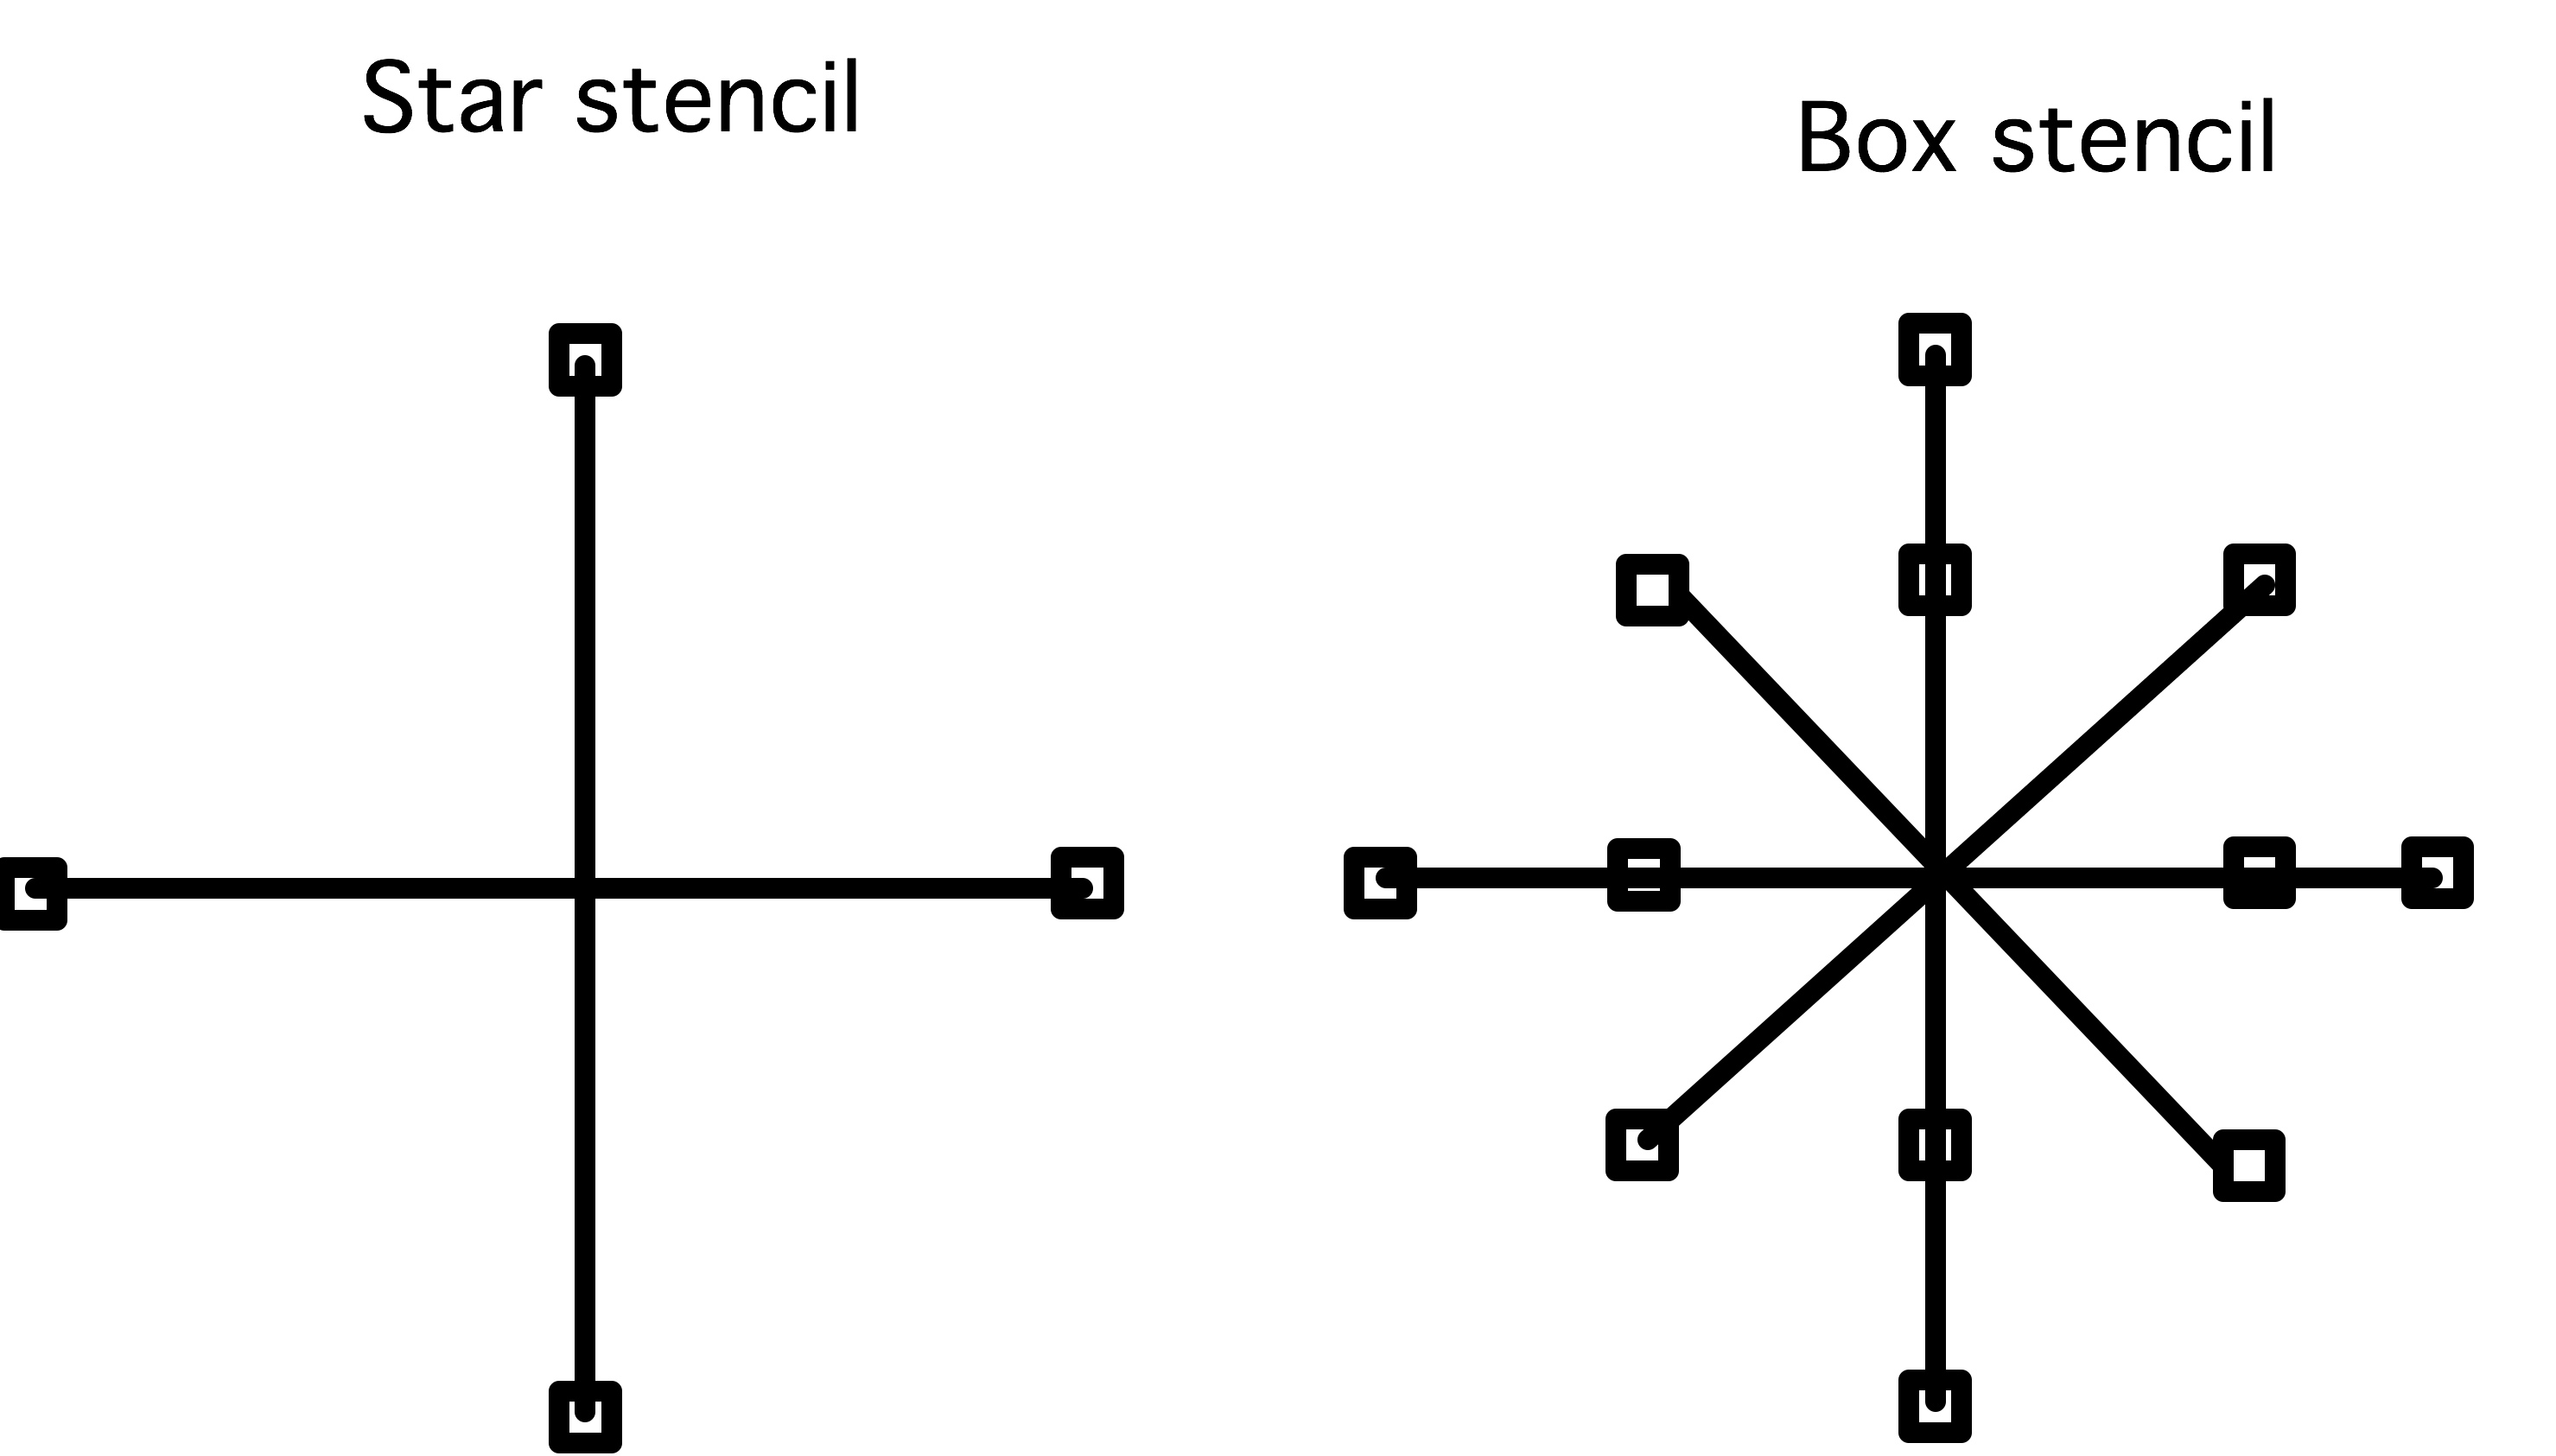
\includegraphics[scale=.5]{starbox}
    \caption{Star and box stencils}
    \label{fig:starbox}
  \end{figure}
  The stencil type is of type \indexpetscdef{DMStencilType},
  with values
  \begin{itemize}
  \item \indexpetscshow{DM_STENCIL_BOX},
  \item \indexpetscshow{DM_STENCIL_STAR}.
  \end{itemize}
  (See figure~\ref{fig:starbox}.)
\item
  The \lstinline{gridx,gridy} values are the global grid size.
  This can easily be set with commandline options
  \indexpetscoption{da_grid_x}\lstinline+/y/z+.
\item
  The \lstinline{procx,procy} variables are an explicit specification
  of the processor grid. Failing this specification, PETSc will try to
  find a distribution similar to the domain grid.
\item \lstinline{dof} indicates the number of `degrees of freedom',
  where 1~corresponds to a scalar problem.
\item \lstinline{width} indicates the extent of the stencil:
  1~for a 5-point stencil or more general a 2nd order stencil
  for 2nd order \acp{PDE},
  2~for 2nd order discretizations of a 4th order \ac{PDE}, et cetera.
\item \lstinline{partitionx,partitiony} are arrays
  giving explicit partitionings of the grid over the processors,
  or \indexpetscshow{PETSC_NULL} for default distributions.
\end{itemize}

After you define a \indexpetscshow{DM} object, each process has a contiguous
subdomain out of the total grid.
You can query its size and location with \indexpetscdef{DMDAGetCorners},
or query that and all other information with \indexpetscref{DMDAGetLocalInfo},
which returns an \indexpetscref{DMDALocalInfo} structure.

(A \indexpetscref{DMDALocalInfo} struct is the same for 1/2/3 dimensions,
so certain fields may not be applicable to your specific \ac{PDE}.)

\begin{figure}[ht]
  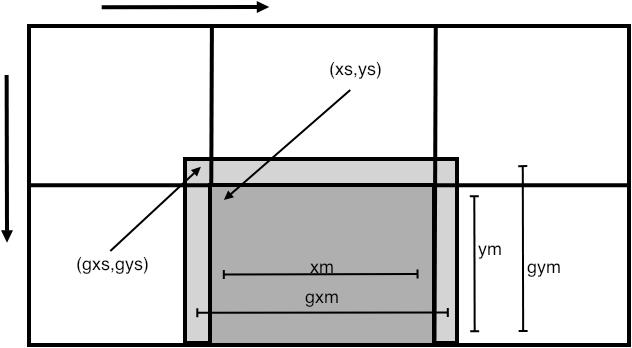
\includegraphics[scale=.3]{dmdalocalinfo}
  \caption{Illustration of various fields of the DMDALocalInfo structure}
  \label{fig:dmdalocalinfo}
\end{figure}

Using the fields in this structure, each process can now iterate over its
own subdomain.
For instance, the `top left' corner of the owned subdomain is at \n{xs,ys}
and the number of points is \n{xm,ym}
(see figure~\ref{fig:dmdalocalinfo}),
so we can iterate over the subdomain as:

\begin{lstlisting}
for (int j=info.ys; j<info.ys+info.ym; j++) {
  for (int i=info.xs; i<info.xs+info.xm; i++) {
    // actions on point i,j
  }
}
\end{lstlisting}

On each point of the domain, we describe the stencil at that point.
First of all, we now have the information to compute the $x,y$ coordinates
of the domain points:
\begin{lstlisting}
PetscReal
  hx = 1. / ( info.mx-1 ),
  hy = 1. / ( info.my-1 );
for (int j=info.ys; j<info.ys+info.ym; j++) {
  for (int i=info.xs; i<info.xs+info.xm; i++) {
    PetscReal x = i*hx, y = j*hy;
    ...
  }
}
\end{lstlisting}

\Level 0 {Constructing a vector on a grid}

A \indexpetscshow{DMDA} object is a description of a grid,
so we now need to concern how to construct a linear system
defined on that grid.

We start with vectors: we need a solution vector
and a right-hand side.
Here we have two options:
\begin{enumerate}
\item we can build a vector from scratch that has the right structure; or
\item we can use the fact that a grid object has a vector that can be extracted.
\end{enumerate}

\Level 1 {Create confirming vector}

If we create a vector with \indexpetscshow{VecCreate} and \indexpetscshow{VecSetSizes},
it is easy to get the global size right, but the default partitioning will
probably not be conformal to the grid distribution.
Also, getting the indexing scheme right is not trivial.

First of all, the local size needs to be set explicitly,
using information from the \indexpetscshow{DMDALocalInfo} object:
%
\cverbatimsnippet{vecdmlocalsize}

After this, you don't use \indexpetscshow{VecSetValues}, but
set elements directly in the raw array, obtained by \indexpetscdef{DMDAVecGetArray}:
%
\cverbatimsnippet{vecdmgetarray}

\Level 1 {Extract vector from DMDA}

\Level 1 {Refinement}

The routine \indexpetscdef{DMDASetRefinementFactor}
can be activated with the options \indexpetscoption{da_refine}
or separately \indexpetscoption{da_refine_x}/y/z for the directions.

\Level 0 {Constructing a matrix on a grid}

\begin{lstlisting}
for (int j=info.ys; j<info.ys+info.ym; j++) {
  for (int i=info.xs; i<info.xs+info.xm; i++) {
    PetscReal x = i*hx, y = j*hy;
    ...
    // set the row, col, v values
    ierr = MatSetValuesStencil(A,1,&row,ncols,col,v,INSERT_VALUES);CHKERRQ(ierr);
  }
}
\end{lstlisting}

Next, we express matrix row/column coordinates in terms of domain coordinates.
The row number corresponds to the $(i,j)$ pair:
\begin{lstlisting}
MatStencil  row;
row.i = i; row.j = j; 
\end{lstlisting}
For a 5-point stencil we need five column numbers,
as well as five element values:
\begin{lstlisting}
MatStencil col[5];
PetscScalar v[5];
PetscInt    ncols = 0;
/**** diagonal element ****/
col[ncols].i = i; col[ncols].j = j;
v[ncols++] = 4.;
\end{lstlisting}

The other `legs' of the stencil need to be set conditionally:
the connection to $(i-1,j)$ is missing on the top row of the domain,
and the connection to $(i,j-1)$ is missing on the left column.
\begin{lstlisting}
/* if not top row */
if (i>0) {
    col[ncols].j = j;   col[ncols].i = i-1;
    v[ncols++] = -1.;
}
/* if not left column */
if (j>0) {
    col[ncols].j = j-1; col[ncols].i = i;
    v[ncols++] = -1.;
}
\end{lstlisting}
Ditto for the connections to $(i+1,j)$ and $(i,j+1)$.

\Level 0 {Vectors of a distributed array}

A distributed array is similar to a distributed vector, so there are routines of
extracting the values of the array in the form of a vector. This can be done in two ways:
of ways.
%
(The routines here actually pertain to the more general \indexpetscshow{DM} `Data Management'
object, but we will for now discuss them in the context of \indexpetscshow{DMDA}.)
%
\begin{enumerate}
\item You can create a `global' vector, defined on the same communicator as the array,
  and which is disjointly partitioned in the same manner. This is done with
  \indexpetscdef{DMCreateGlobalVector}:
\begin{lstlisting}
PetscErrorCode DMCreateGlobalVector(DM dm,Vec *vec)    
\end{lstlisting}
\item You can create a `local' vector,
  which is sequential and defined on \indexpetscshow{PETSC_COMM_SELF},
  that has not only the points local to the process, but also the `halo' region
  with the extent specified in the definition of the \clstinline{DMDACreate} call.
  For this, use \indexpetscdef{DMCreateLocalVector}:
\begin{lstlisting}
PetscErrorCode DMCreateLocalVector(DM dm,Vec *vec)
\end{lstlisting}
\end{enumerate}

Values can be moved between local and global vectors by:
\begin{itemize}
\item \indexpetscdef{DMGlobalToLocal}: this establishes a local vector,
  including ghost/halo points from a disjointly distributed global vector.
  (For overlapping communication and computation, use
  \indexpetscdef{DMGlobalToLocalBegin} and \indexpetscdef{DMGlobalToLocalEnd}.)
\item \indexpetscdef{DMLocalToGlobal}: this copies the disjoint parts
  of a local vector back into a global vector.
  (For overlapping communication and computation use
  \indexpetscdef{DMLocalToGlobalBegin} and \indexpetscdef{DMLocalToGlobalEnd}.)
\end{itemize}

\Level 0 {Matrices of a distributed array}

Once you have a grid, can create its associated matrix:
\begin{lstlisting}
DMSetUp(grid);
DMCreateMatrix(grid,&A)
\end{lstlisting}

With this subdomain information you can then start to create the coefficient matrix:
\begin{lstlisting}
DM grid;
PetscInt i_first,j_first,i_local,j_local;
DMDAGetCorners(grid,&i_first,&j_first,NULL,&i_local,&j_local,NULL);
for ( PetscInt i_index=i_first; i_index<i_first+i_local; i_index++) {
  for ( PetscInt j_index=j_first; j_index<j_first+j_local; j_index++) {
  // construct coefficients for domain point (i_index,j_index)
  }
}
\end{lstlisting}
Note that indexing here is in terms of the grid, not in terms of the matrix.

For a simple example, consider 1-dimensional smoothing.
From \indexpetscshow{DMDAGetCorners} we need only the parameters in $i$-direction:
%
\cverbatimsnippet[examples/petsc/c/grid1d.c]{dmda1corners}

We then use a single loop to set elements for the local range in $i$-direction:
%
\cverbatimsnippet[examples/petsc/c/grid1d.c]{dmda1stencil}

